\documentclass[a4paper,14pt]{extarticle}

% -------------------------------------
%                Пакеты
% -------------------------------------
\usepackage{geometry}
\geometry{a4paper,tmargin=2cm,bmargin=2cm,lmargin=3cm,rmargin=1cm}

\usepackage[T2A]{fontenc}
\usepackage[utf8]{inputenc}
\usepackage[english, main=russian]{babel}

\usepackage{textcomp}
\usepackage{indentfirst}
\usepackage{graphicx}
\graphicspath{{./images/}}
\usepackage{enumitem}
\usepackage{caption}
\usepackage{hyperref}
\hypersetup{unicode=true}

\DeclareCaptionLabelSeparator*{emdash}{~--- }
\captionsetup[figure]{labelsep=emdash,font=onehalfspacing,position=bottom}

\usepackage{tempora}
\usepackage{amsmath}
\usepackage{color}
\usepackage{listings}

\lstset{
  belowcaptionskip=1\baselineskip,
  breaklines=true,
  frame=L,
  xleftmargin=\parindent,
  language=C++,
  showstringspaces=false,
  basicstyle=\footnotesize\ttfamily,
  keywordstyle=\bfseries\color{blue},
  commentstyle=\itshape\color{purple},
  identifierstyle=\color{black},
  stringstyle=\color{red},
  numbers=left,
  numberstyle=\tiny,
  stepnumber=1,
  numbersep=5pt
}

\linespread{1.3}
\sloppy
\clubpenalty=10000
\widowpenalty=10000

% -------------------------------------
%               Документ
% -------------------------------------
\begin{document}

% -------------------------------------
%           Титульный лист
% -------------------------------------
\begin{titlepage}
\thispagestyle{empty}

\vspace*{-60pt}
\begin{center}
  
\includegraphics[width=0.35\textwidth]{emblem}
\end{center}

\vspace{-25pt}
\hrule height2.3pt
\vspace*{-20.3pt}
\hrule

\vspace{4ex}
\begin{center}
  \small
  Министерство науки и высшего образования Российской Федерации\\
  Федеральное государственное бюджетное образовательное учреждение высшего образования\\
  «МГТУ им.~Н.\,Э.~Баумана (НИУ)»
\end{center}

\vspace{11em}
\begin{center}
  \Large\bfseries Летучка AruCo
\end{center}

\vspace{8em}
\begin{flushright}
  Студент группы ИУ9-21Б \textbf{Хромов М.\,А.}\\[2ex]
  Преподаватель \textbf{Посевин Д.\,П.}
\end{flushright}

\vfill
\begin{center}
  \textsl{Москва 2025}
\end{center}
\end{titlepage}

% -------------------------------------
\section{Задание — часть 1}
\begin{enumerate}[nosep]
  \item Реализовать пример \texttt{detect\_markers.cpp} на OpenCV + ArUco.
  \item Вывести в консоль координаты \emph{углов} найденных меток ArUco.
\end{enumerate}

% -------------------------------------
\section{Задание — часть 2}
Реализовать одну из трёх задач, перечисленных в п.~2.  
Для летучки выбран вариант \emph{«Определение позы человека»}  
(детекция скелета с использованием DNN-модели MPI).

% -------------------------------------
\section{Код программ}\label{sect:listings}
Все исходники поделены на части не длиннее 70 строк и отделены
командой \verb|\clearpage|.

% ----------  Листинг 1-а  ----------
\begin{figure}[!htb]
\begin{lstlisting}[caption={\texttt{detect_aruco.cpp}, строки 1–70},label={lst:aruco-a},firstnumber=1,lastline=70]
#include <opencv2/opencv.hpp>
#include <opencv2/aruco.hpp>
#include <iostream>
#include <unistd.h>
#include <limits.h>

int main() {
    char cwd[PATH_MAX];
    if (getcwd(cwd,sizeof(cwd)))
        std::cout << "Working directory: " << cwd << std::endl;

    cv::VideoCapture cap(0);
    if (!cap.isOpened()) {
        std::cerr << "Ошибка: не удалось открыть камеру!\n";
        return -1;
    }
    std::cout << "Камера открыта. 'q' или Esc — выход.\n";

    auto dictionary = cv::aruco::getPredefinedDictionary(
                          cv::aruco::DICT_4X4_1000);
    auto params = cv::aruco::DetectorParameters::create();
    params->adaptiveThreshConstant   = 7;
    params->minMarkerPerimeterRate   = 0.01;
    params->maxMarkerPerimeterRate   = 4.0;
    params->adaptiveThreshWinSizeMin = 3;
    params->adaptiveThreshWinSizeMax = 23;
    params->adaptiveThreshWinSizeStep= 10;

    while (true) {
        cv::Mat frame;  cap >> frame;
        if (frame.empty()) {
            cv::Mat ph = cv::Mat::zeros(480,640,CV_8UC3);
            cv::putText(ph,"No Camera Frame",{50,50},
                        cv::FONT_HERSHEY_SIMPLEX,1.0,{255,255,255},2);
            cv::imshow("ArUco Detection",ph);
            char k = (char)cv::waitKey(30);
            if (k=='q' || k==27) break;
            continue;
        }
\end{lstlisting}
\end{figure}
\clearpage

% ----------  Листинг 1-б  ----------
\begin{figure}[!htb]
\begin{lstlisting}[caption={\texttt{detect_aruco.cpp}, окончание},label={lst:aruco-b},firstnumber=71]
        cv::Mat gray;
        cv::cvtColor(frame,gray,cv::COLOR_BGR2GRAY);

        std::vector<int> ids;
        std::vector<std::vector<cv::Point2f>> corners;
        cv::aruco::detectMarkers(gray,dictionary,corners,ids,params);

        if (!ids.empty()) {
            std::cout << "--- Найдено " << ids.size()
                      << " маркер(ов) ---\n";
            for (size_t i=0;i<ids.size();++i) {
                std::cout << "ID=" << ids[i] << " :";
                for (auto& p: corners[i])
                    std::cout << " (" << p.x << "," << p.y << ")";
                std::cout << '\n';
            }
            cv::aruco::drawDetectedMarkers(frame,corners,ids);
        }
        cv::imshow("ArUco Detection",frame);
        char key=(char)cv::waitKey(30);
        if (key=='q' || key==27) break;
    }
    cap.release();
    cv::destroyAllWindows();
    return 0;
}
\end{lstlisting}
\end{figure}
\clearpage

% ----------  Листинг 2-а  ----------
\begin{figure}[!htb]
\begin{lstlisting}[caption={\texttt{pose_estimation.cpp}, строки 1–70},label={lst:pose-a},firstnumber=1,lastline=70]
#include <opencv2/opencv.hpp>
#include <opencv2/dnn.hpp>
#include <iostream>

using namespace cv;
using namespace dnn;
using namespace std;

const int PAIRS[14][2] = {
    {0,1},{1,2},{2,3},{3,4},{1,5},
    {5,6},{6,7},{1,14},{14,8},{8,9},
    {9,10},{14,11},{11,12},{12,13}
};

int main() {
    string proto  ="pose/mpi/pose_deploy_linevec_faster_4_stages.prototxt";
    string model  ="pose/mpi/pose_iter_160000.caffemodel";
    int nPoints = 15;

    Net net = readNetFromCaffe(proto,model);
    net.setPreferableBackend(DNN_BACKEND_OPENCV);
    net.setPreferableTarget (DNN_TARGET_CPU);

    VideoCapture cap(0);
    if (!cap.isOpened()) {
        cerr << "Ошибка: нет веб-камеры\n"; return -1;
    }

    int inW=368,inH=368; float thr=0.1;
    while (waitKey(1)<0) {
        Mat frame; cap>>frame; if (frame.empty()) break;
        Mat blob=blobFromImage(frame,1./255,Size(inW,inH),
                               Scalar(0,0,0),false,false);
        net.setInput(blob);
        Mat out = net.forward();
\end{lstlisting}
\end{figure}
\clearpage

% ----------  Листинг 2-б  ----------
\begin{figure}[!htb]
\begin{lstlisting}[caption={\texttt{pose_estimation.cpp}, окончание},label={lst:pose-b},firstnumber=71]
        int H=out.size[2], W=out.size[3];
        vector<Point> pts(nPoints);

        for(int n=0;n<nPoints;++n){
            Mat prob(H,W,CV_32F,out.ptr(0,n));
            Point maxLoc; double prob;
            minMaxLoc(prob,0,&prob,0,&maxLoc);
            if(prob>thr){
                int x=frame.cols*maxLoc.x/W;
                int y=frame.rows*maxLoc.y/H;
                pts[n]=Point(x,y);
                circle(frame,{x,y},6,Scalar(0,255,255),-1);
                putText(frame,to_string(n),{x,y},
                        FONT_HERSHEY_SIMPLEX,0.5,Scalar(0,0,255),1);
            }
        }
        for(int i=0;i<14;++i){
            Point A=pts[PAIRS[i][0]], B=pts[PAIRS[i][1]];
            if(A.x>0 && B.x>0)
                line(frame,A,B,Scalar(0,255,0),2);
        }
        imshow("Pose Estimation",frame);
    }
    return 0;
}
\end{lstlisting}
\end{figure}
\clearpage

% -------------------------------------
\section{Реализация — скриншоты}
\begin{center}
  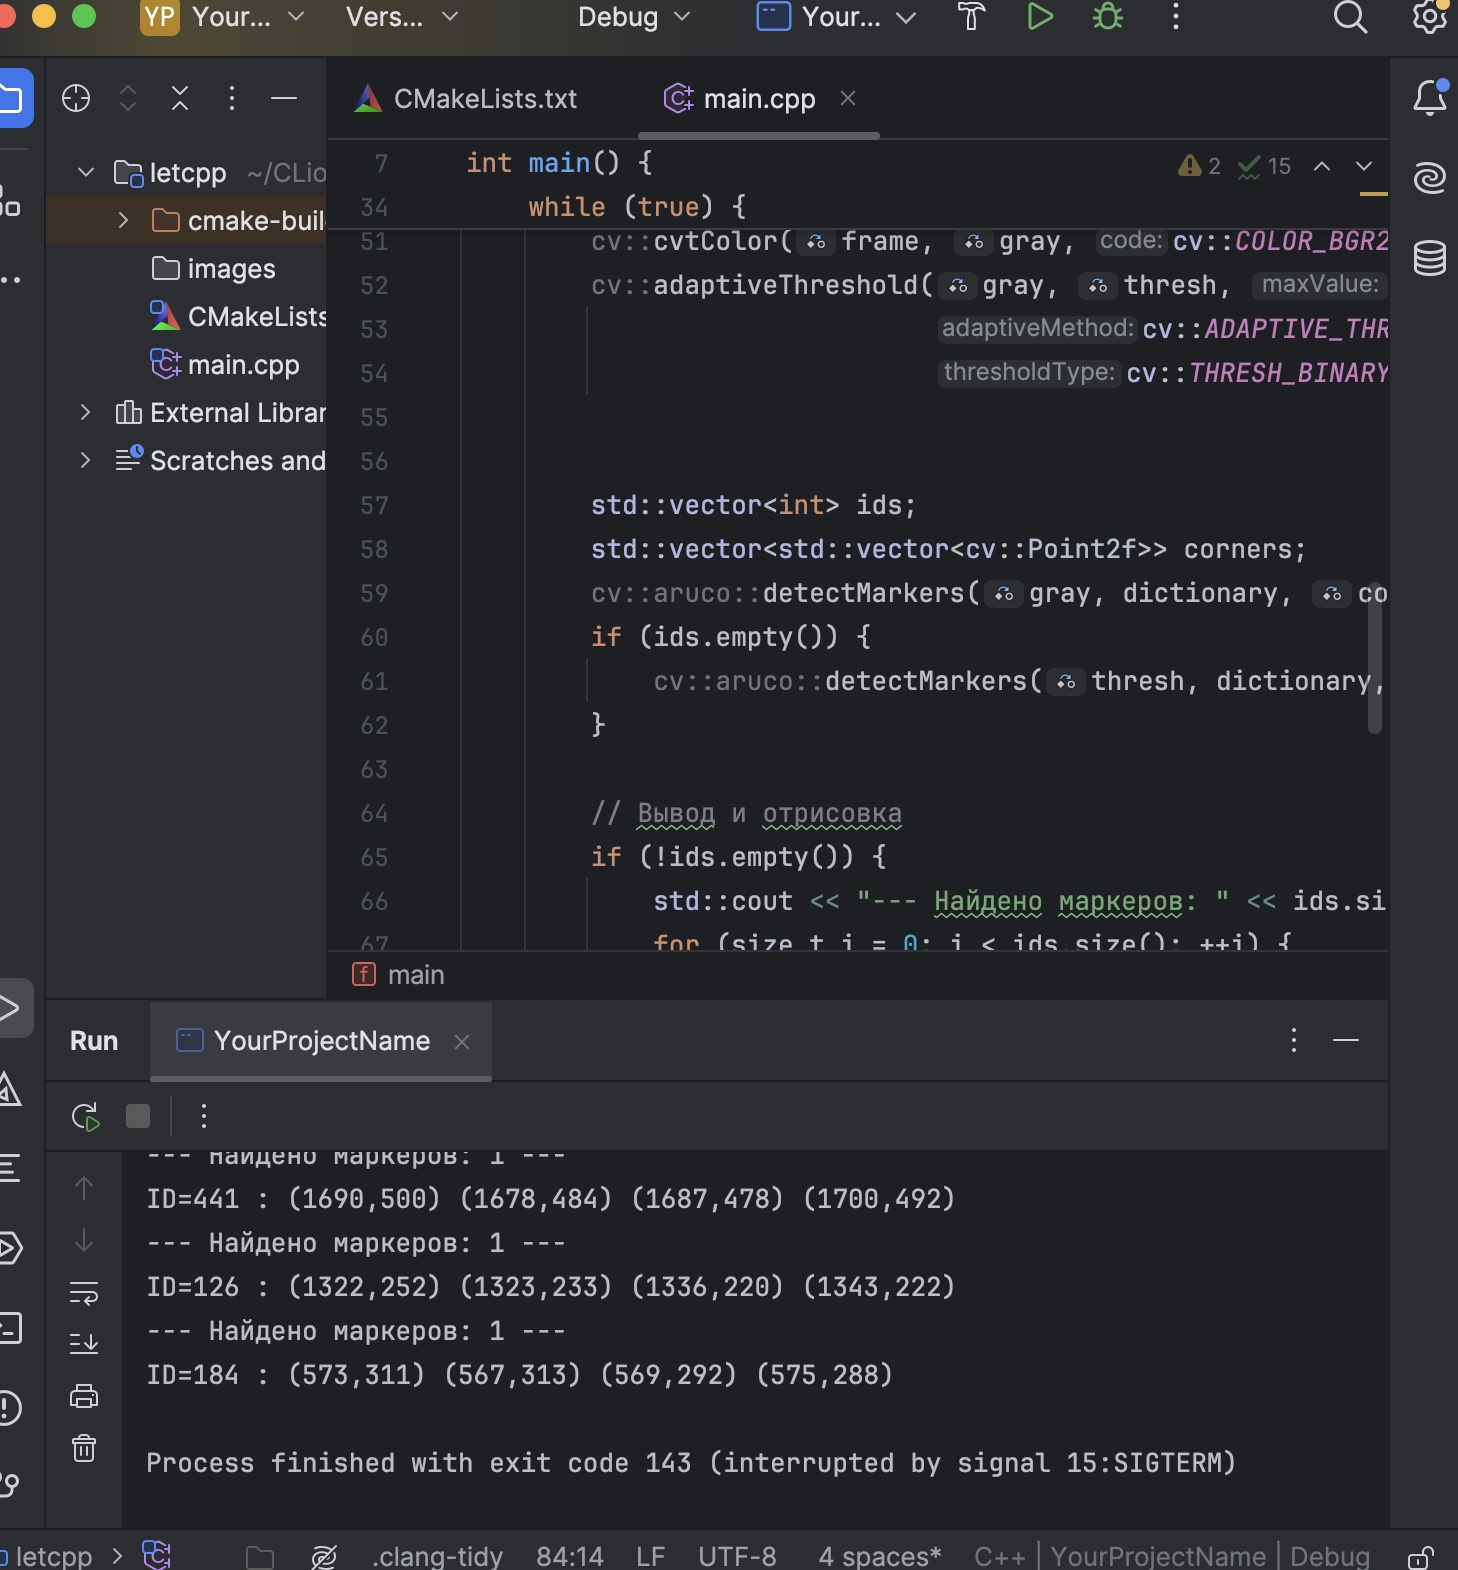
\includegraphics[width=0.8\textwidth]{фото26.jpeg}
  \captionof{figure}{Работа детектора ArUco-меток}
\end{center}

\begin{center}
  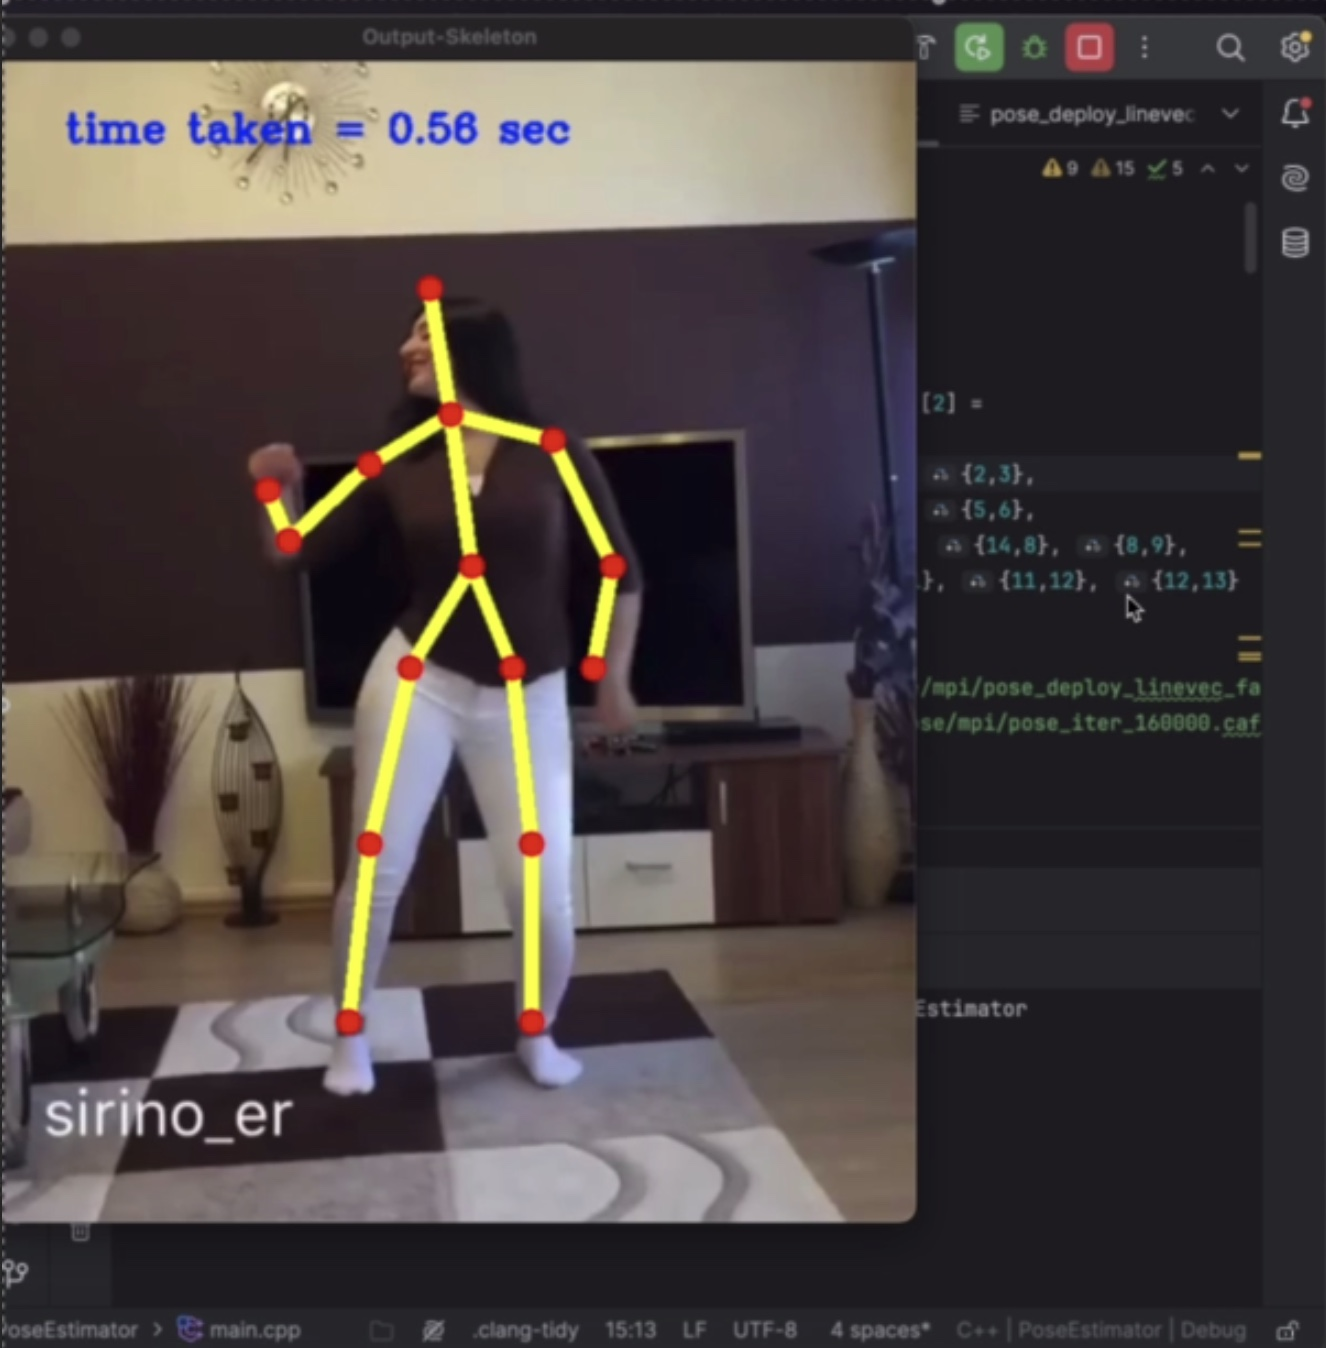
\includegraphics[width=0.8\textwidth]{фото27.jpeg}
  \captionof{figure}{Определение позы человека (MPI model)}
\end{center}

% -------------------------------------
\section{Вывод}
В ходе «Летучки AruCo» были выполнены две самостоятельные под-задачи:

\begin{itemize}[nosep]
  \item \textbf{Часть 1.} Реализован пример \texttt{detect\_markers.cpp}.  
        Программа определяет ID меток ArUco в реальном времени,
        выводя в консоль координаты всех четырёх углов
        каждой найденной метки и визуализируя результат
        поверх видеопотока.
  \item \textbf{Часть 2.} Реализована модель определения позы человека
        (скелет) на базе сети MPI-I в OpenCV DNN.  
        Для каждого кадра выводятся ключевые точки и рёбра скелета;
        решение закрепляет навык работы с DNN-модулем и графикой OpenCV.
\end{itemize}

Обе задачи демонстрируют владение современными инструментами
компьютерного зрения: работа с камерой, DNN-инференс, ArUco-метки,
а также умение выводить отладочную информацию для анализа результатов.
\end{document}
